\documentclass[10pt,dvipdfmx,cjk]{beamer}
%% 基本のbeamerテーマ設定を読み込む
\usepackage{styles/mytheme}
%% 必要な設定を読み込む
\usepackage{styles/mysetting}

%% タイトル
\title[title CambridgeUS]{
  CambridgeUS のシンプル設定
}
\subtitle{
  ロゴも入る
}
\author[お名前]{あなたのお名前\inst{1}}
\institute[所属]{\inst{1}所属している団体名(1人なら\texttt{\textbackslash inst\{1\}}は不要)}
\date[日付]{発表する研究集会情報や日付など}

\titlegraphic{\flushright%
  %\transparent{0.4} % 透かしを入れたい場合はコメントアウト
  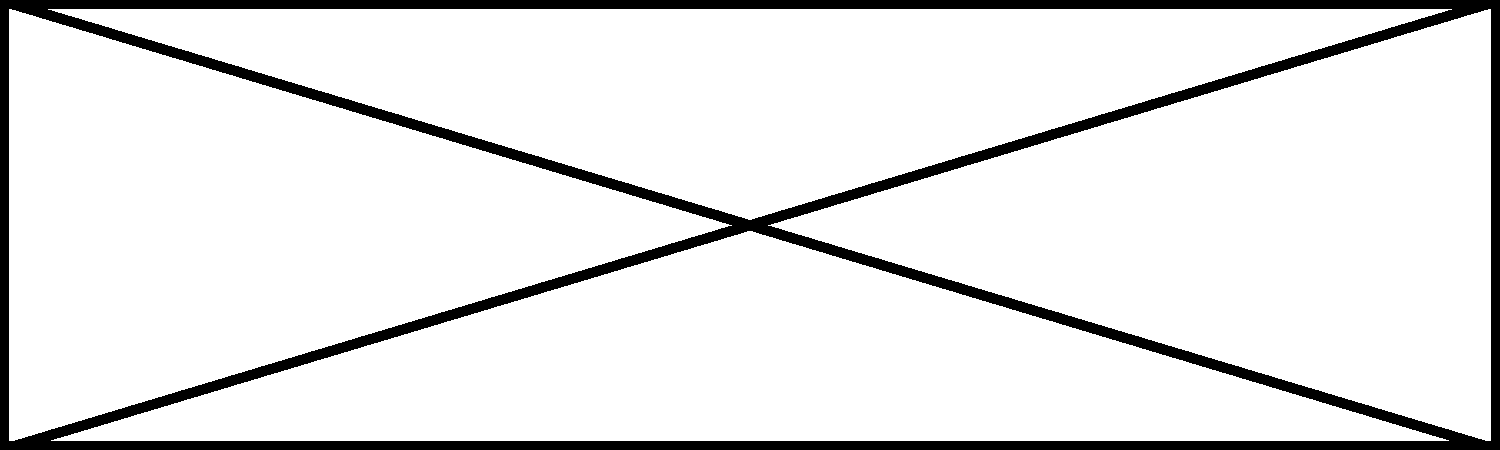
\includegraphics[height=25pt]{dummy_logo_black.png}%
}

%% 節先頭毎に目次を追加
\AtBeginSection[]{
  \begin{frame}[noframenumbering,plain]{\insertsectionhead}{}
    \tableofcontents[currentsection]
  \end{frame}
}

%% ここから本文
\begin{document}
  %% タイトル
  \begin{frame}[noframenumbering,plain]{}{}
    \titlepage
  \end{frame}

  %% 目次
  \begin{frame}[noframenumbering,plain]{目次}{}
    \tableofcontents%[hideallsubsections]
  \end{frame}

  \section{最初の節}
  \begin{frame}{はじめの1歩}
    Beamer で作った PDF は, 全画面表示やプレゼンモードで使っていく.
    詰め込まないようにした方が綺麗に見える.
    詰め込むときは, 図示や{\scriptsize 文字サイズ}など工夫した方が良い.
    聴講者や発表会場によっても文字サイズは変わってくるかもしれない.

    \[
      \begin{tikzcd} % & を\& にすること!
        \mathscr{A} \arrow[d]\arrow[rd,"\iota_\mathscr{A}^{}"]\\
        \mathscr{D}b \arrow[r,"\iota_{\mathscr{D}b}^{}"] \& \mathscr{B}.
      \end{tikzcd}
    \]

    \pause % より詳細な設定ができる\only,\uncover,\visibleなどもある
    \begin{dfn}[定義の名前 $\ast$ 無くてもよい]
      任意の$a\in\mathbb{R}$に対して, 次が成り立つ.
      \[
        a^2 \geq 0.
      \]
    \end{dfn}

    \vspace{1.2em} % 1.2 文字分 縦に 隙間を追加. マイナスもできる. 前に区切り文字を入れないとたまにおかしくなる.
    より詳しくは\,
    参考になる文献\footnote[1]{\cite{book:dummy}著者. 本のタイトル. 出版社, 出版年1900.}
    を参照.
  \end{frame}

  \section{次の節}
  \begin{frame}{その他の色確認}{}
    \begin{columns}
      \begin{column}[t]{0.5\textwidth-0.01\textwidth}
        箇条書き(\texttt{\textbackslash itemize})
        \begin{itemize}
          \item 最初
          \item 真ん中
          \item 最後
        \end{itemize}
      \end{column}
      \begin{column}[t]{0.5\textwidth-0.01\textwidth}
        \ruby{箇条}{か|じょう}書き(\texttt{\textbackslash enumerate})
        \begin{enumerate}[(i)]
          \item 最初
          \item 真ん中
          \item 最後
        \end{enumerate}
      \end{column}
    \end{columns}
  
    \begin{block}{block title}
      block body
    \end{block}
    \begin{alertblock}{alertblock title}
      alertblock body
    \end{alertblock}
    \begin{exampleblock}{exampleblock title}
      exampleblock body
    \end{exampleblock}
  \end{frame}

  %% 参考文献
  \section*{参考文献}
  \begin{frame}[noframenumbering,plain]{参考文献}{}
    \bibliography{ref}
  \end{frame}
\end{document}